\chapter{Decision Trees}\label{chap:dectrees}

\section{Introduction}

Given a set of training data in the form of input-output pairs, supervised learning enables the prediction of a new example given only as the inputs ~\cite{aimp17}. In this chapter we will be focusing on decision trees, a supervised learning algorithm, and investigate how it performs given our data.

\section{Input model}
\par
A decision tree requires the input data to be a fixed number of input features. We therefore need to model our data a bit more. In order to be able to use a decision tree model to classify our data, we must change our model to one that enables us to extract discrete features that characterise the path taken by the person inside the airport. The general idea is to process the readings in such a way, that in the end we will be left with a list of sensors to which the device was closest, ordered by time, therefore representing a trajectory.\\

\par
In \ref{chap:datamodelling} we filled out the table in a linear fashion:

\begin{align*}
    T_{s_kt_k} := c_k, \quad \forall (t_k, c_k, s_k) \in \mathcal{X}_i 
\end{align*}

For the decision tree, we will change this to:

\begin{align*}
    T_{s_k\log_{1.1} t_k} := c_k, \quad \forall (t_k, c_k, s_k) \in \mathcal{X}_i 
\end{align*}
    
\par
The reason for this is minimising information loss while reducing the length of the table. Most of our addresses spend less than 30 minutes in the airport, but, since there are staff addresses that spend up to 8 hours, we would need to make all tables be the same size. Applying $log_{1.1}$ results in us keeping high detail for the first half hour, and less for everything after. Practically, considering the reading resolution is one second, we will need 75 rows for the first 30 minutes, while 110 rows cover the full 8 hours a staff might spend in the area. Therefore our fixed length can be 110, instead of the 28800 rows (8*60*60) otherwise needed.\\

\par
We can now easily form a list of length 110 of the closest sensors to the device, which we will call $PROG$, which we populate thus:

\begin{align*}
    PROG_i = \max_{s_k} (T_{s_ki}),\quad s_k \in S, i \in [0, 110]
\end{align*}

Which, if we continue the processing of the data in \cref{fig:datamodelling:tables:3} on page  \pageref{fig:datamodelling:tables}, will result in
\begin{align*}
    [S1, S1, S1, S1, S1, S1, S1, S2, S2, S3, S3]
\end{align*}

which represents a chronologically ordered list of the sensors closest to the Bluetooth address. In other words, for each discrete timestamp in the table, we pick the sensor that has the highest reading out of all of them. So if at timestamp $t$ we have

\begin{figure}[H]
    \centering
    \begin{tabular}{ |c||c|c|c| }
         \hline
         timestamp & S1 & S2 & S3 \\
         \hline
         ...  & ... & ... & ... \\ 
         t & -50 & -74 & -43 \\ 
         ... & ... & ... & ... \\ 
         \hline
    \end{tabular}
    % just edit the three \subcaption
    % also you can use \subcaption instead of \subcaption* if you want them to be labelled (a, b, c by default), this can for sure be changed
    % \subcaption{Step 1}
    \label{fig:dectrees:selectingexample}
\end{figure}

we would pick S3 at index t of PROG. This enables us to have a discrete representation of the path a Bluetooth address took through the airport.\\

\par
We can then assign each item in $PROG$ as a distinct input feature to our decision tree, so that input feature $I_i = PROG_i$.

\section{Principles}

Decision trees (or classification trees) are simple ways of classifying examples. The tree is a binary tree consisting of conditions as internal nodes and results as leaves. In order to classify a new input on a created tree, one simply filters it down the tree based on the conditions, and returns the leaf at the end of the path.
\begin{figure}[H]
    \centering
    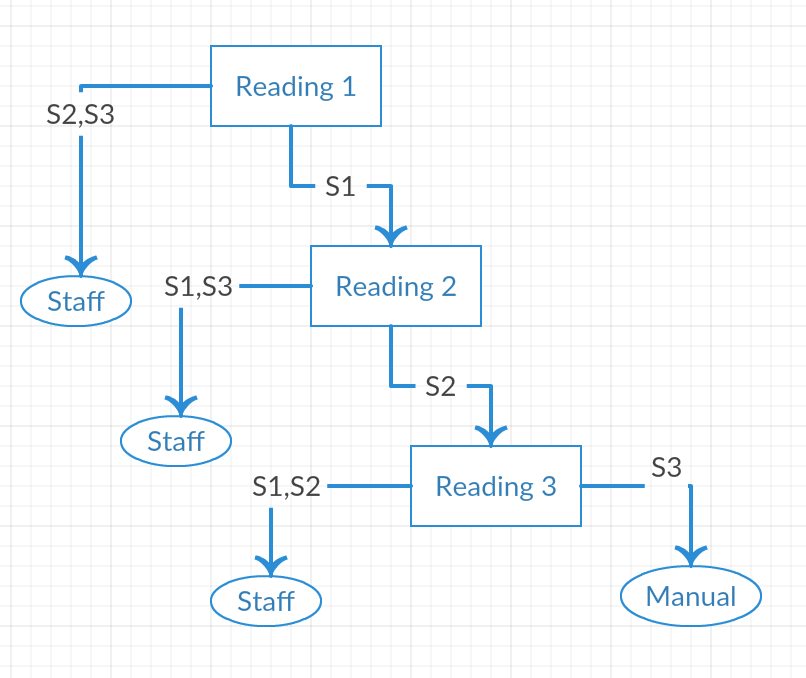
\includegraphics[scale=0.5]{Pictures/dectree.png}
    \caption{Example of a decision tree that classifies the probability of an address being "Staff" or "Manual"}
    \label{fig:dectree}
\end{figure}

In order to learn a decision tree, a splitting condition must be found. The algorithm does this by calculating the expected entropy for each condition and picking the lowest one, thus maximising information gain. \cite{tdndectrees}\\

\par
We first calculate the entropy for each potential condition using
\begin{align*}
	Entropy(S) = -\sum_c p_{(c)} \log_2p_{(c)}
\end{align*}

where $p_{(c)}$ is the frequency of examples of class c in S

%TODO example with table and calculations of entropy


% BEGIN RESULT EVAL %

\section{Evaluating the results}

The methodology is as follows: In the seven days of data, we have
\begin{itemize}
	\item manual - 3574 addresses 
	\item staff - 8045 addresses
	\item no-q - 1633 addresses
	\item privium - 278 addresses
\end{itemize}

Training and testing will be done on a 66\%/34\% train/test split on the whole dataset. We will thus create the tables

\begin{itemize}
	\item train - 8930 addresses 
	\item test  - 4600 addresses
\end{itemize}

The model is trained using the train dataset, then the testing dataset is evaluated using the trained model. Afterwards we compare the predicted labels with the true labels and create the resulting confusion matrix below, that breaks down the performance of the model:


\begin{figure}[H]
    \centering
    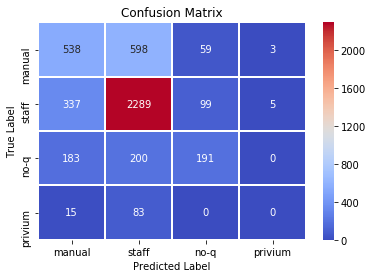
\includegraphics[width=.5\textwidth]{Pictures/decision_tree_confusion.png}
    \caption{Decision tree results (confusion matrix)}
    \label{fig:dectrees:confusion_matrix}
\end{figure}

\subsection{Performance summary}

As described in \ref{section:performance_metrics}, below is the performance summary for decision trees on our data, derived from the confusion matrix in Figure \ref{fig:dectrees:confusion_matrix}. 

\begin{table}[H]
    \centering 
    \begin{tabular}{c|c|c|c|}
        \cline{2-4}
                                                     & \textbf{Precision} & \textbf{Recall} & \textbf{Examples} \\ \hline
        \multicolumn{1}{|l|}{\textbf{manual}}        & 0.50               & 0.45            & 1198              \\ \hline
        \multicolumn{1}{|l|}{\textbf{staff}}         & 0.72               & 0.84            & 2730              \\ \hline
        \multicolumn{1}{|l|}{\textbf{no-q}}          & 0.55               & 0.33            & 574               \\ \hline
        \multicolumn{1}{|l|}{\textbf{privium}}       & 0.00               & 0.00            & 98                \\ 
        \hline \hline
        \multicolumn{1}{|l|}{\textbf{Average / Total}} & 0.44               & 0.40            & 4600               \\ 
        \hline \hline
        \multicolumn{1}{|l|}{\textbf{Accuracy}}      & \multicolumn{3}{c|}{0.66}                                \\ \hline
    \end{tabular}   
    \caption{Performance summary for decision trees}
\end{table}
\subsection{Interpretation and Conclusion}
This approach has yielded far better results than label propagation did, but its accuracy is still unsatisfactory. The reason for this is mostly due to inconsistencies in readings, with many parameters affecting signal strengths: other people, location of the Bluetooth device, owner's rotation, etc. In the end, the difference between keeping the device in the left or right pocket might be interpreted differently by our algorithm due to the line of sight to the different sensors, and this could potentially have an impact on the results. \par
\medskip
Another effect of this is that it is difficult to line the timelines up. A device might be picked up by a sensor far before another one, so their timelines, although similar, will be offset. This is incompatible with the current approach, where, ideally, we hope all devices to be in the same spot at $t_0$.\par
\medskip
We have therefore decided that decision trees are not the way to go either, and will continue trying to find other algorithms that can learn to ignore such irregularities.